% This file was created by matlab2tikz.
%
%The latest updates can be retrieved from
%  http://www.mathworks.com/matlabcentral/fileexchange/22022-matlab2tikz-matlab2tikz
%where you can also make suggestions and rate matlab2tikz.
%
\definecolor{mycolor1}{rgb}{0.85000,0.95000,1.00000}%
\definecolor{mycolor2}{rgb}{0.95000,0.85000,0.85000}%
\definecolor{mycolor3}{rgb}{0.06600,0.44300,0.74500}%
\definecolor{mycolor4}{rgb}{0.12941,0.12941,0.12941}%
%
\begin{tikzpicture}

\begin{axis}[%
width=\textwidth,
height=0.252\textheight,
at={(0\textwidth,0\textheight)},
scale only axis,
xmin=0,
xmax=59,
xlabel style={font=\color{mycolor4}},
xlabel={Time (s)},
ymin=0,
ymax=52.5,
ylabel style={font=\color{mycolor4}},
ylabel={Packets/s},
axis background/.style={fill=white},
axis x line*=bottom,
axis y line*=left,
xmajorgrids,
ymajorgrids,
grid=both,
tick align=outside,
scaled y ticks=true,
title style={yshift=1.0ex}
]

\addplot[area legend, draw=none, fill=mycolor1, fill opacity=0.35, forget plot]
table[row sep=crcr] {%
x	y\\
13	0\\
23	0\\
23	52.5\\
13	52.5\\
}--cycle;

\addplot[area legend, draw=none, fill=mycolor2, fill opacity=0.25, forget plot]
table[row sep=crcr] {%
x	y\\
38	0\\
45	0\\
45	52.5\\
38	52.5\\
}--cycle;
\addplot [color=mycolor3, forget plot]
  table[row sep=crcr]{%
0	0\\
5	0\\
6	1\\
7	0\\
8	2\\
9	0\\
10	1\\
11	14\\
12	11\\
13	11\\
14	10\\
15	12\\
17	10\\
18	12\\
20	10\\
21	2\\
23	0\\
24	2\\
26	0\\
27	2\\
29	2\\
30	3\\
32	1\\
33	3\\
35	1\\
36	3\\
37	2\\
38	2\\
39	3\\
40	0\\
41	1\\
43	1\\
44	0\\
59	0\\
};
\end{axis}
\end{tikzpicture}%